\section*{Ziel}
Ziel des Versuchs ist es, die Fourier-Transformation kennenzulernen. 
Hierzu wird zum Einen eine bekannte periodische Funktion durch Fourier-Transformation in die Elementarschwingung zerlegt und 
zum Anderen eine periodische Funktion aus Elementarschwingungen gebildet.
\section{Theorie}
\label{sec:theorie}
\subsection{Fourier-Reihenentwicklung, harmonische Analyse}
\label{sec:theorie1}
Für eine T-periodische Funktion $F$ der Zeit gilt
\begin{equation}
	F(t) = F(t+\mathup{T}) \qquad\forall t, 
\end{equation}
für eine Q-periodische Funktion $G$ des Ortes gilt
\begin{equation}
	G(x) = G(x+Q) \qquad\forall x. 
\end{equation}
Nach dem Fourier'schen Theorem lassen sich solche periodischen Funktionen, etwa Wellenfunktionen $F(x,t)$, als Linearkombination aus den Elementarschwingungen
\begin{alignat}{3}
	a_\text{n}\text{sin}\Bigl(\frac{2π}{\mathup{T}}t\Bigr) &\qquad\text{und} &&\qquad b_\text{n}\text{cos}\Bigl(\frac{2π}{\mathup{T}}t\Bigr)
\end{alignat}
zusammenfügen.
Das bedeutet, dass die Reihe
\begin{equation}
	\frac{a_0}{2}+\sum_{n=1}^\infty \Bigl(a_\text{n}\text{sin}(\underbrace{n\frac{2π}{\mathup{T}}}_{\omega}t) 
	+ b_\text{n}\text{cos}(\underbrace{n\frac{2π}{\mathup{T}}}_{\omega}t) \Bigr)
	\label{eq:reihe}
\end{equation}
mit $\omega=2\mathup{\pi}\cdot f$
eine T-periodische Funktion $f$ der Zeit darstellt, sofern die Reihe konvergent ist.
Gleichmäßige Konvergenz der Fourier-Reihe ist gegeben, wenn die Funktion $F$ auf ihrem Definitionsbereich stetig ist.

Für die Koeffizienten in \ref{eq:reihe} gilt
\begin{subequations}
\begin{equation}
	a_\text{n} = \frac{2}{\text{T}}\int_0^\text{T} F(t)\text{cos}(2n\mathup{\pi}t)dt
	\label{eq:koeff1}
\end{equation}
\begin{equation}
	b_\text{n} = \frac{2}{\text{T}}\int_0^\text{T} F(t)\text{sin}(2n\mathup{\pi}t)dt.
	\label{eq:koeff2}
\end{equation}
\label{eq:koeff}
\end{subequations}
Die Schwingung wird für $n=0$ Grundschwingung und die Schwingungen für $n>1$ Oberschwingungen bezeichnet.
Für gerade Funktionen $F$, also mit $F(x)=F(-x)$, sind alle $b_\text{n}=0$; 
analog sind für ungerade Funktionen $F$, also mit $-F(x)=F(-x)$, alle $a_\text{n}=0$.

Durch diese Formeln ist allgemein das Beschreiben einer T-periodischen Funktion als konvergente Fourier-Reihe möglich.
Dies wird als harmonische Analyse oder Fourier-Analyse bezeichnet.
\subsection{Linienspektrum der Frequenzen, Spektralanalyse}
\label{sec:theorie2}
Werden die Fourier-Koeffizienten in Gleichungen \eqref{eq:koeff} als Funktionen der Frequenzen $f$ aufgetragen, so ergeben sich Frequenzspektren. 
In diesen ist abgezeichnet, aus welchen Elementarschwingungen die Funktion $F$ besteht und welchen Wert die Fourier-Koeffizienten \eqref{eq:koeff} aufweisen.
\begin{figure}
	\centering
	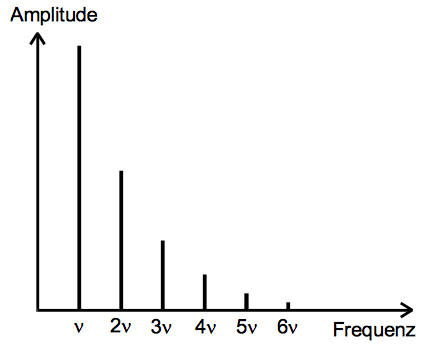
\includegraphics[width=0.4\textwidth]{Bilder/Linienspektrum.png}
	\caption{Beispiel eines Frequenzspektrums bei konvergenter Fourier-Reihe. \cite{V351}}
	\label{fig:analyse}
\end{figure}
Bei konvergenten Fourier-Reihen \eqref{eq:reihe} geht die Höhe der diskreten Linien für $f\xrightarrow{}\infty$ gegen Null.

\subsection{Nicht-periodische Funktionen, Fourier-Transformation}
\label{sec:theorie3}
Nicht-periodische Funktionen $F$ zeigen bei Spektralanalyse \ref{fig:analyse} ein kontinuierliches Spektrum, weiter gilt nicht $a_\text{n},b_\text{n}\xrightarrow{f\to\infty}0$ im Allgemeinen.
Für diese Funktionen ohne konvergenten Fourier-Reihen wird eine Fourier-Transformation angewandt.


